\PassOptionsToPackage{unicode=true}{hyperref} % options for packages loaded elsewhere
\PassOptionsToPackage{hyphens}{url}
\PassOptionsToPackage{dvipsnames,svgnames*,x11names*}{xcolor}
%
\documentclass[8pt,ignorenonframetext,dvipsnames]{beamer}
\usepackage{pgfpages}
\setbeamertemplate{caption}[numbered]
\setbeamertemplate{caption label separator}{: }
\setbeamercolor{caption name}{fg=normal text.fg}
\beamertemplatenavigationsymbolsempty
% Prevent slide breaks in the middle of a paragraph:
\widowpenalties 1 10000
\raggedbottom
\setbeamertemplate{part page}{
\centering
\begin{beamercolorbox}[sep=16pt,center]{part title}
  \usebeamerfont{part title}\insertpart\par
\end{beamercolorbox}
}
\setbeamertemplate{section page}{
\centering
\begin{beamercolorbox}[sep=12pt,center]{part title}
  \usebeamerfont{section title}\insertsection\par
\end{beamercolorbox}
}
\setbeamertemplate{subsection page}{
\centering
\begin{beamercolorbox}[sep=8pt,center]{part title}
  \usebeamerfont{subsection title}\insertsubsection\par
\end{beamercolorbox}
}
\AtBeginPart{
  \frame{\partpage}
}
\AtBeginSection{
  \ifbibliography
  \else
    \frame{\sectionpage}
  \fi
}
\AtBeginSubsection{
  \frame{\subsectionpage}
}
\usepackage{lmodern}
\usepackage{amssymb,amsmath}
\usepackage{ifxetex,ifluatex}
\usepackage{fixltx2e} % provides \textsubscript
\ifnum 0\ifxetex 1\fi\ifluatex 1\fi=0 % if pdftex
  \usepackage[T1]{fontenc}
  \usepackage[utf8]{inputenc}
  \usepackage{textcomp} % provides euro and other symbols
\else % if luatex or xelatex
  \usepackage{unicode-math}
  \defaultfontfeatures{Ligatures=TeX,Scale=MatchLowercase}
\fi
% use upquote if available, for straight quotes in verbatim environments
\IfFileExists{upquote.sty}{\usepackage{upquote}}{}
% use microtype if available
\IfFileExists{microtype.sty}{%
\usepackage[]{microtype}
\UseMicrotypeSet[protrusion]{basicmath} % disable protrusion for tt fonts
}{}
\IfFileExists{parskip.sty}{%
\usepackage{parskip}
}{% else
\setlength{\parindent}{0pt}
\setlength{\parskip}{6pt plus 2pt minus 1pt}
}
\usepackage{xcolor}
\usepackage{hyperref}
\hypersetup{
            pdftitle={Introduction to Multivariate Regression \& Program Evaluation},
            pdfauthor={Lecture 11},
            colorlinks=true,
            linkcolor=Maroon,
            filecolor=Maroon,
            citecolor=Blue,
            urlcolor=blue,
            breaklinks=true}
\urlstyle{same}  % don't use monospace font for urls
\newif\ifbibliography
\usepackage{graphicx,grffile}
\makeatletter
\def\maxwidth{\ifdim\Gin@nat@width>\linewidth\linewidth\else\Gin@nat@width\fi}
\def\maxheight{\ifdim\Gin@nat@height>\textheight\textheight\else\Gin@nat@height\fi}
\makeatother
% Scale images if necessary, so that they will not overflow the page
% margins by default, and it is still possible to overwrite the defaults
% using explicit options in \includegraphics[width, height, ...]{}
\setkeys{Gin}{width=\maxwidth,height=\maxheight,keepaspectratio}
\setlength{\emergencystretch}{3em}  % prevent overfull lines
\providecommand{\tightlist}{%
  \setlength{\itemsep}{0pt}\setlength{\parskip}{0pt}}
\setcounter{secnumdepth}{0}

% set default figure placement to htbp
\makeatletter
\def\fps@figure{htbp}
\makeatother


%packages
\usepackage{graphicx}
\usepackage{rotating}
\usepackage{hyperref}

\usepackage{tikz} % used for text highlighting, amongst others
\usepackage{comment}

%title slide stuff
%\institute{Department of Education}
%\title{Managing and Manipulating Data Using R}

%
\setbeamertemplate{navigation symbols}{} % get rid of navigation icons:
\setbeamertemplate{footline}[page number]

%\setbeamertemplate{frametitle}{\thesection \hspace{0.2cm} \insertframetitle}
\setbeamertemplate{section in toc}[sections numbered]
%\setbeamertemplate{subsection in toc}[subsections numbered]
\setbeamertemplate{subsection in toc}{%
  \leavevmode\leftskip=3.2em\color{gray}\rlap{\hskip-2em\inserttocsectionnumber.\inserttocsubsectionnumber}\inserttocsubsection\par
}

%define colors
%\definecolor{uva_orange}{RGB}{216,141,42} % UVa orange (Rotunda orange)
\definecolor{mygray}{rgb}{0.95, 0.95, 0.95} % for highlighted text
	% grey is equal parts red, green, blue. higher values >> lighter grey
	%\definecolor{lightgraybo}{rgb}{0.83, 0.83, 0.83}

% new commands

%highlight text with very light grey
\newcommand*{\hlg}[1]{%
	\tikz[baseline=(X.base)] \node[rectangle, fill=mygray] (X) {#1};%
}
%, inner sep=0.3mm
%highlight text with very light grey and use font associated with code
\newcommand*{\hlgc}[1]{\texttt{\hlg{#1}}}

%modifying back ticks to add grey background
\let\OldTexttt\texttt
\renewcommand{\texttt}[1]{\OldTexttt{\hlg{#1}}}


\begin{comment}

% Font
\usepackage[defaultfam,light,tabular,lining]{montserrat}
\usepackage[T1]{fontenc}
\renewcommand*\oldstylenums[1]{{\fontfamily{Montserrat-TOsF}\selectfont #1}}

% Change color of boldface text to darkgray
\renewcommand{\textbf}[1]{{\color{darkgray}\bfseries\fontfamily{Montserrat-TOsF}#1}}

% Bullet points
\setbeamertemplate{itemize item}{\color{BlueViolet}$\circ$}
\setbeamertemplate{itemize subitem}{\color{BrickRed}$\triangleright$}
\setbeamertemplate{itemize subsubitem}{$-$}

% Reduce space before lists
%\addtobeamertemplate{itemize/enumerate body begin}{}{\vspace*{-8pt}}

\let\olditem\item
\renewcommand{\item}{%
  \olditem\vspace{4pt}
}

% decreasing space before and after level-2 bullet block
%\addtobeamertemplate{itemize/enumerate subbody begin}{}{\vspace*{-3pt}}
%\addtobeamertemplate{itemize/enumerate subbody end}{}{\vspace*{-3pt}}

% decreasing space before and after level-3 bullet block
%\addtobeamertemplate{itemize/enumerate subsubbody begin}{}{\vspace*{-2pt}}
%\addtobeamertemplate{itemize/enumerate subsubbody end}{}{\vspace*{-2pt}}

%Section numbering
\setbeamertemplate{section page}{%
    \begingroup
        \begin{beamercolorbox}[sep=10pt,center,rounded=true,shadow=true]{section title}
        \usebeamerfont{section title}\thesection~\insertsection\par
        \end{beamercolorbox}
    \endgroup
}

\setbeamertemplate{subsection page}{%
    \begingroup
        \begin{beamercolorbox}[sep=6pt,center,rounded=true,shadow=true]{subsection title}
        \usebeamerfont{subsection title}\thesection.\thesubsection~\insertsubsection\par
        \end{beamercolorbox}
    \endgroup
}

\end{comment}

\title{Introduction to Multivariate Regression \& Program Evaluation}
\providecommand{\subtitle}[1]{}
\subtitle{HED 612}
\author{Lecture 11}
\date{}

\begin{document}
\frame{\titlepage}

\begin{frame}
\tableofcontents[hideallsubsections]
\end{frame}
\begin{frame}{Where are we going\ldots{}.}
\protect\hypertarget{where-are-we-going.}{}

\begin{itemize}
\tightlist
\item
  This Lecture

  \begin{itemize}
  \tightlist
  \item
    Other OLS assumptions
  \item
    Creating publication quality tables
  \item
    Review:

    \begin{itemize}
    \tightlist
    \item
      Cabrera, N. L., Milem, J. F., Jaquette, O., \& Marx, R. (2014).
      Missing the (student achievement) forest for all the (political)
      trees: Empiricism and the Mexican American Studies controversy in
      Tucson. American Educational Research Journal, 51(6), 1084-1118.
    \end{itemize}
  \end{itemize}
\item
  Next Lecture

  \begin{itemize}
  \tightlist
  \item
    Introduction to non-linear relationships between X and Y
  \item
    Mini lesson on what each section of manuscrupt should accomplish!
  \item
    Review:

    \begin{itemize}
    \tightlist
    \item
      Powers, J. M. (2004). High-Stakes Accountability and Equity: Using
      Evidence From California's Public Schools Accountability Act to
      Address the Issues in Williams v. State of California. American
      Educational Research Journal, 41(4), 763--795.
    \end{itemize}
  \end{itemize}
\end{itemize}

\end{frame}

\hypertarget{final-projects}{%
\section{Final Projects}\label{final-projects}}

\begin{frame}{Final Projects are optional}
\protect\hypertarget{final-projects-are-optional}{}

\begin{itemize}
\tightlist
\item
  \textbf{Final projects are optional}
\item
  You can decide to not move forward with your final project:

  \begin{itemize}
  \tightlist
  \item
    Don't feel ``guilty'' for not being able to complete this project
  \item
    I already know you are all brilliant scholars, practitioners,
    educators!
  \item
    Prioritize your health (physical \& mental), loved ones\ldots{}
  \end{itemize}
\item
  You can decide to move forward with your final project:

  \begin{itemize}
  \tightlist
  \item
    If you have the time/ability to do it and do it for your own
    professional development!
  \item
    Send me an email to set up our first Zoom meeting to discuss RQ,
    topic, and data
  \item
    We will set up a timeline
  \item
    I will help you clean the data!
  \end{itemize}
\end{itemize}

\end{frame}

\hypertarget{ols-assumptions}{%
\section{OLS Assumptions}\label{ols-assumptions}}

\begin{frame}{OLS Assumptions}
\protect\hypertarget{ols-assumptions-1}{}

\begin{enumerate}
\tightlist
\item
  The conditional assumption of \(u_i\) given \(X_i\) has a mean a zero
\item
  (\(X_i\), \(Y_i\)), \(i=1, ...n\) are independently and identically
  distributed (i.i.d)
\item
  Large outliers are unlikely
\item
  Homoskedasticity
\end{enumerate}

\medskip

\begin{itemize}
\tightlist
\item
  If these assumptions hold:

  \begin{itemize}
  \tightlist
  \item
    Then our OLS estimators, \(\hat{\beta_0}\) and \(\hat{\beta_1}\)
    have normal distributions in large samples
  \item
    And because they have normal distributions, we can use
    \(\hat{\beta_0}\) and \(\hat{\beta_1}\) to test hypothesess about
    the population parameters \(\beta_0\) and \(\beta_1\)
  \end{itemize}
\item
  If these assumptions are violated:

  \begin{itemize}
  \tightlist
  \item
    We produced inefficeint and biased estimates, \(\hat{\beta_0}\) and
    \(\hat{\beta_1}\), of the population parameters \(\beta_0\) and
    \(\beta_1\)
  \end{itemize}
\end{itemize}

\end{frame}

\begin{frame}{First OLS Assumption}
\protect\hypertarget{first-ols-assumption}{}

\begin{enumerate}
\tightlist
\item
  \textbf{The conditional assumption of \(u_i\) given \(X_i\) has a mean
  a zero}
\end{enumerate}

\begin{itemize}
\tightlist
\item
  What does this mean?

  \begin{itemize}
  \tightlist
  \item
    The independent variable \(X_i\) is unrelated to all variables that
    were not included in the model (i.e., \(u_i\))
  \item
    If we violate this assumption, we produce a biased estimate!
  \item
    What's a biased estimate? Consistenly overestimating or
    underestimating population parameter! {[}remember Lec 9?{]}
  \item
    If \(u_i\) given \(X_i\) has a mean a zero = our predictions do not
    systematically over or underestimate, thus balance out to zero = no
    bias!
  \end{itemize}
\item
  Thus far we have learned ``simple regression'' (i.e., one independent
  variable of interest) with a major flaw:

  \begin{itemize}
  \tightlist
  \item
    We ignore other ``determinants'' (i.e., control variables) of the
    dependent variable that correlate with our one independent variable
    of interest
  \item
    Remember that other ``determinants'' or ``other variables that
    impact the dependent'' variable that are not in our model are
    collected in the residual term \(u_i\), which we have thus far
    \emph{assumed} to be unrelated with the independent variable of
    interest
  \item
    If we exclude these other determinants that are related to our
    independent variable of interest; we introduce estimation bias via
    an omitted variable!
  \end{itemize}
\item
  \textbf{Omitted Variable Bias}

  \begin{itemize}
  \tightlist
  \item
    Why does omitted variable bias violate OLS Assumption 1?
  \item
    What happens when you omit a ``Z'' variable from your model? It is
    absorbed by the residual term!
  \item
    We know that the ``Z'' variable omitted from the model is correlated
    to our independent variable of interest, which now means that our X
    is not uncorrelated to the residual = violation of OLS 1!
  \end{itemize}
\end{itemize}

\end{frame}

\begin{frame}{First OLS Assumption cont.}
\protect\hypertarget{first-ols-assumption-cont.}{}

\begin{itemize}
\tightlist
\item
  Practical Example: What is the effect number of years of schooling on
  income? 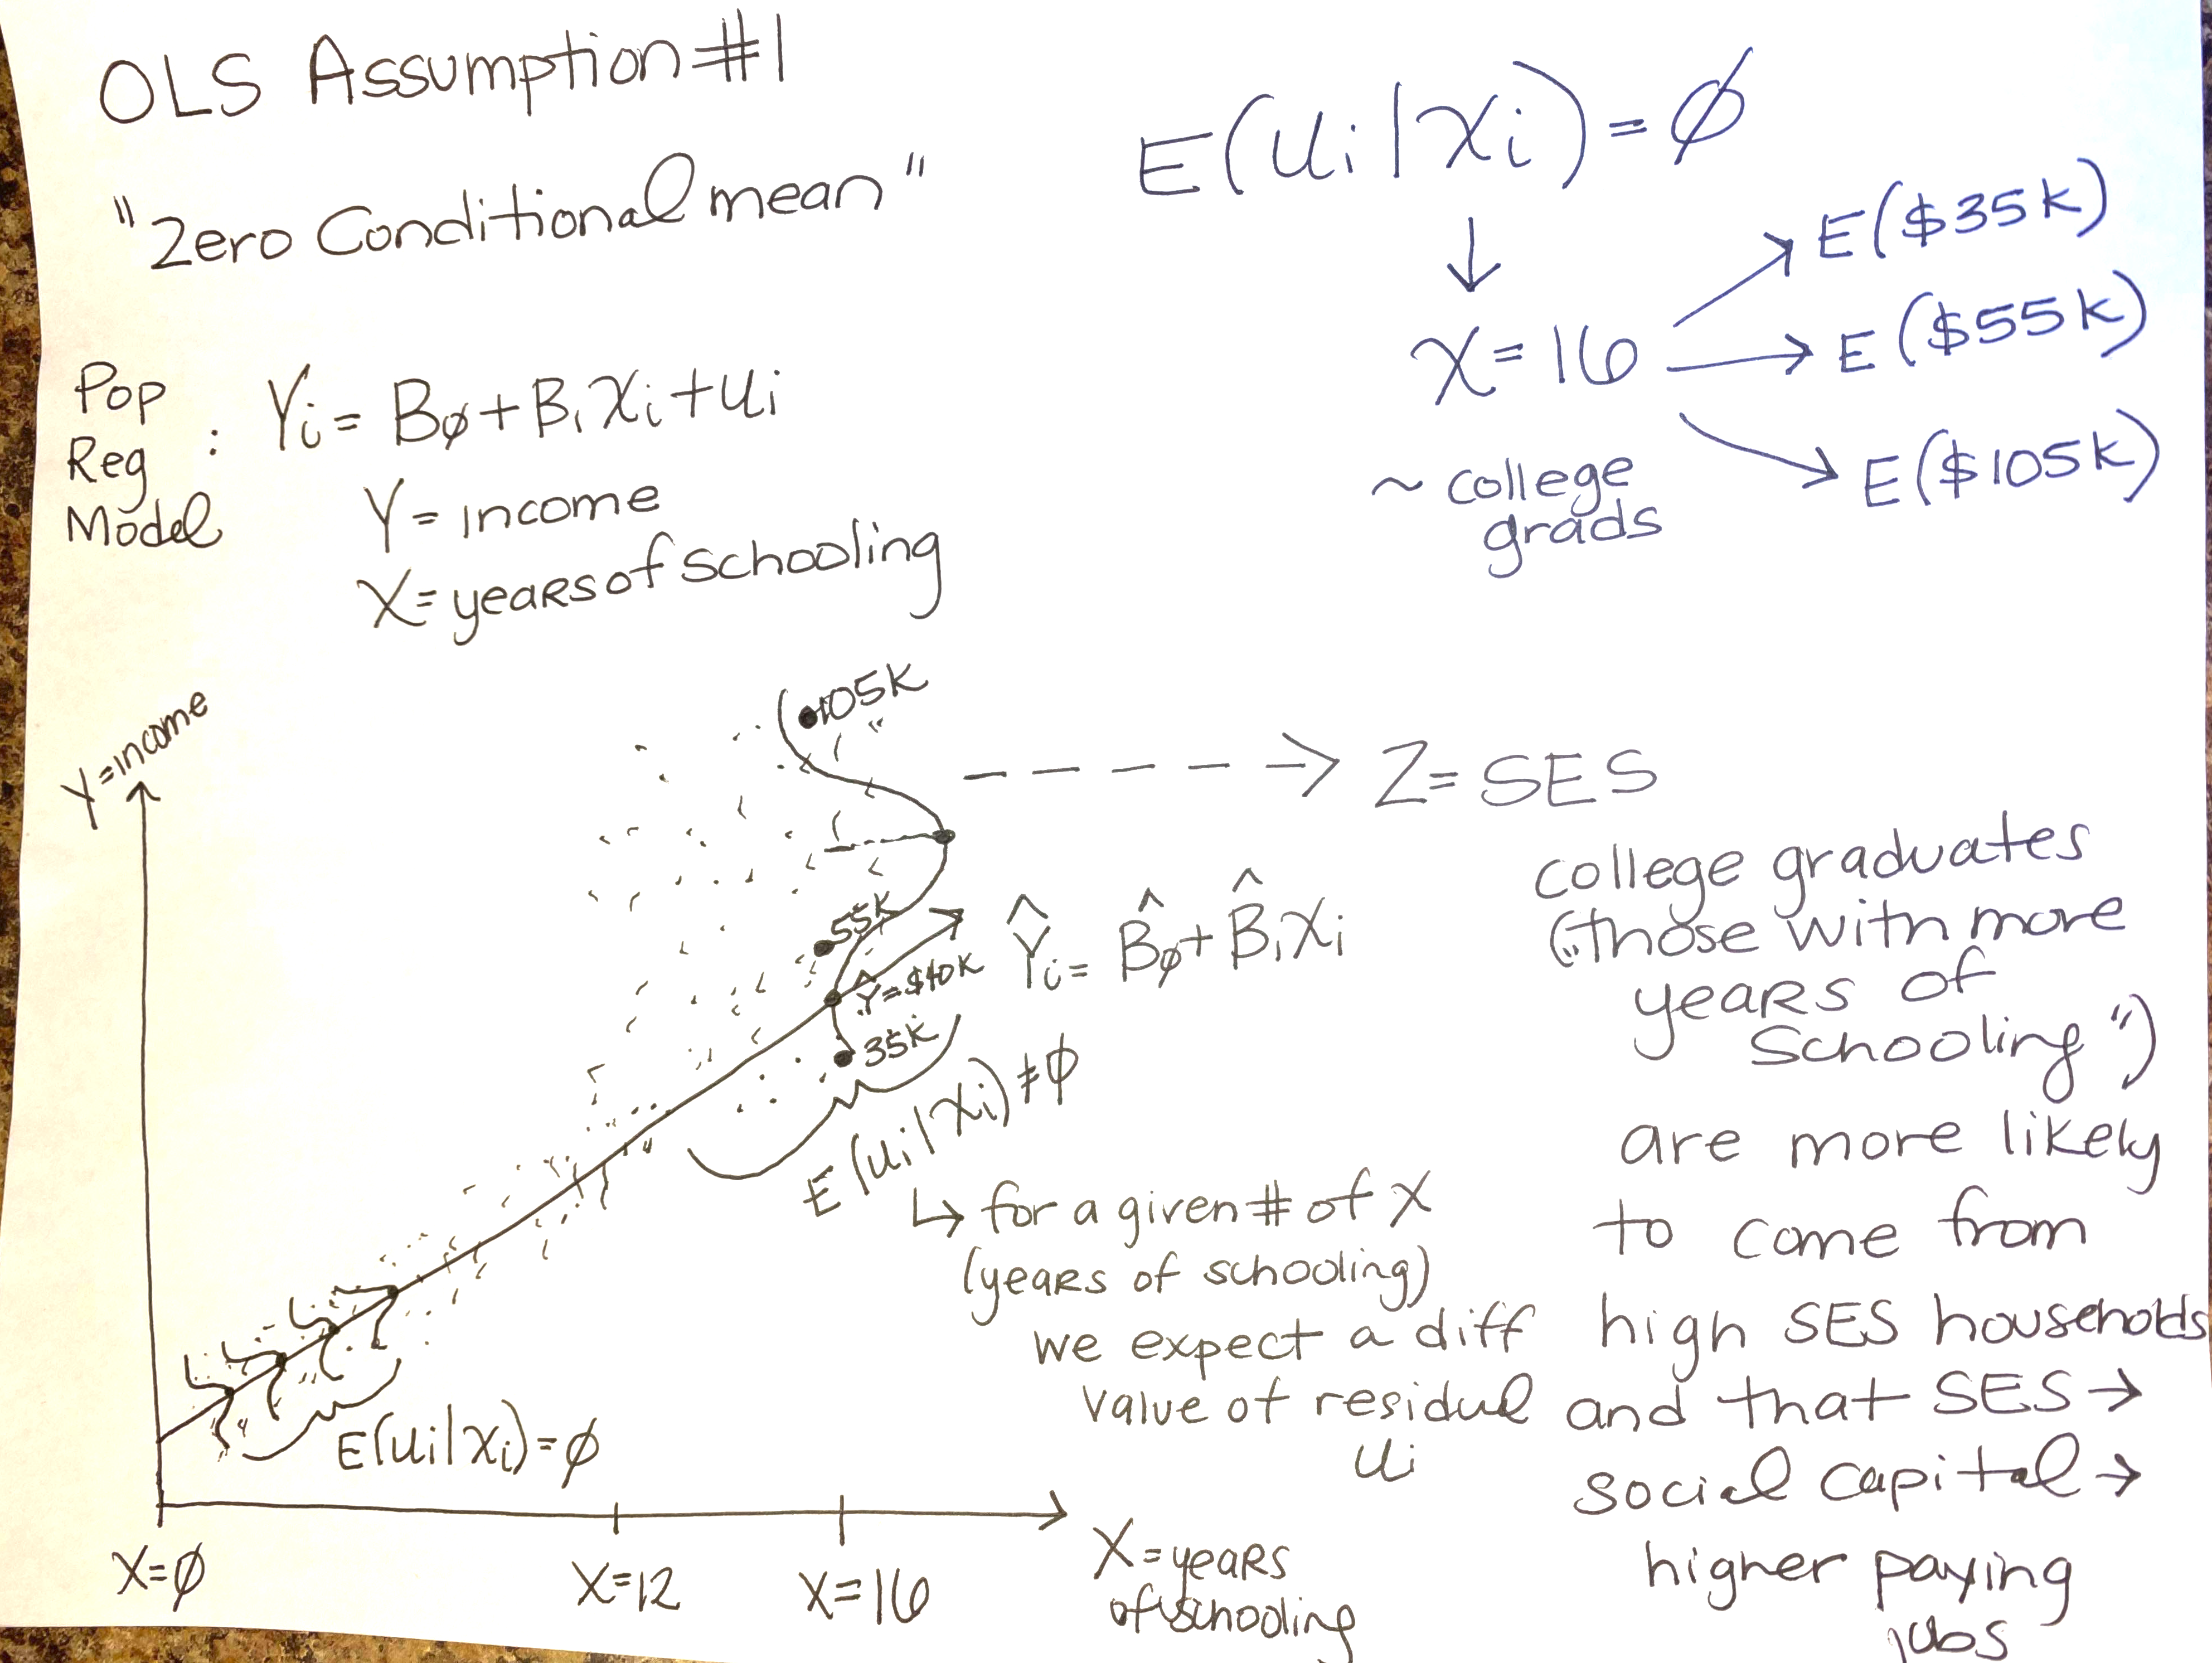
\includegraphics{ols1.png}
\end{itemize}

\end{frame}

\begin{frame}{First OLS Assumption cont}
\protect\hypertarget{first-ols-assumption-cont}{}

\begin{itemize}
\tightlist
\item
  Practical Example: What is the effect number of years of schooling on
  income?
\item
  \(Y_i = \beta_0 + \beta_1X_i +u_1\)
\item
  There are lots of other factors that would influence income besides
  years of schooling!

  \begin{itemize}
  \tightlist
  \item
    If we don't include them in the regression as control variables,
    they are thus relegated to the \(u_1\) and we assume they are not
    systematically related to years of schooling.
  \item
    If this excluded variable meets both conditions of omitted variable
    bias (Z affects Y and Z is related to X); then there is a systematic
    relationship and should not be in the residual!
  \item
    \textbf{By keeping it in the residual (i.e., excluding it from the
    model), we violate OLS Assumption 1 and produce a biased estimate!}
  \end{itemize}
\end{itemize}

\medskip

In practice, OLS Assumption 1 is the most difficult to prove and the
most important for program evaluation research!

\begin{itemize}
\tightlist
\item
  We can draw on the conditional independence assumption:

  \begin{itemize}
  \tightlist
  \item
    Once we include relevant control variables; there are no omitted
    variables that affect Y and have a systematic relationship with X
  \item
    Meaning, if we satisfy the conditional independent assumption
    through control variables, then multiple regression is just as good
    as random assignment experiment (the gold standard of program
    evaluation!)
  \end{itemize}
\end{itemize}

\end{frame}

\begin{frame}{Second OLS Assumption}
\protect\hypertarget{second-ols-assumption}{}

\begin{enumerate}
\setcounter{enumi}{1}
\tightlist
\item
  \textbf{(\(X_i\), \(Y_i\)), \(i=1, ...n\) are independently and
  identically distributed (i.i.d)}
\end{enumerate}

\begin{itemize}
\tightlist
\item
  What does this mean?

  \begin{itemize}
  \tightlist
  \item
    This is about sampling!
  \end{itemize}
\end{itemize}

\medskip

\emph{(\(X_i\), \(Y_i\)), \(i=1, ...n\) are independently distributed}

\begin{itemize}
\tightlist
\item
  Knowing that observation i takes on particular values for X and Y
  tells you nothing about the probability of the next observation taking
  on particular values for X and Y
\item
  When is assumption of independently distributed violated?

  \begin{itemize}
  \tightlist
  \item
    Longitudinal data: knowing a data point in one time period tells you
    something about a data point in another time period

    \begin{itemize}
    \tightlist
    \item
      Ex: Amount of \$ student received via a Federal Pell Grant
      freshman year at UA probably tells you something about how much \$
      student received via a Federal Pell Grant sophmore year at UA
    \end{itemize}
  \item
    Hierarchical data:

    \begin{itemize}
    \tightlist
    \item
      Ex: Students are nested within classrooms. Knowing the reading
      test score of one student in a classroom is probably correlated
      with reading test score for another student in the same classroom.
    \end{itemize}
  \end{itemize}
\end{itemize}

\end{frame}

\begin{frame}{Second OLS Assumption cont.}
\protect\hypertarget{second-ols-assumption-cont.}{}

\emph{(\(X_i\), \(Y_i\)), \(i=1, ...n\) are identically distributed}

\begin{itemize}
\tightlist
\item
  Prior to choosing sample of observations for the population, the
  probability distribution (i.e., the likelihood that \(Y_i\) takes on
  certain values) is the same for all observation
\item
  This is always true if you take a random sample!

  \begin{itemize}
  \tightlist
  \item
    One randomly selected observation has the same probability of taking
    on a certain value of \(Y_i\) as another randomly selected
    observation
  \end{itemize}
\item
  When is the assumption of identically distributed violated?

  \begin{itemize}
  \tightlist
  \item
    Sampling bias:

    \begin{itemize}
    \tightlist
    \item
      Ex: You want to investigate probability of being tardy to college
      lectures and take a sample of students living on campus. Sampling
      bias: you did not include commuter students. If you were to
      randomly select a student living on campus, they are not likely to
      have the same probability of being tardy to lecture than a
      randomly selected commuter student.
    \end{itemize}
  \end{itemize}
\end{itemize}

\end{frame}

\begin{frame}{Third OLS Assumption}
\protect\hypertarget{third-ols-assumption}{}

\begin{enumerate}
\setcounter{enumi}{2}
\tightlist
\item
  Large outliers are unlikely
\end{enumerate}

\begin{itemize}
\tightlist
\item
  Outliers: observations with values of \(X_i\) and \(Y_i\) that are
  outside the ``usual'' range of the data
\item
  Outliers will affect your regression coefficients!
\item
  Stock and Watson have a very technical, mathematical definition of
  when this likely; but in practice this is about really
  investigating/knowing your data
\item
  In practice, if you do find outliers:

  \begin{itemize}
  \tightlist
  \item
    Be sure the data is entered correctly and cleaned

    \begin{itemize}
    \tightlist
    \item
      Ex: Survey data codes missing data as very unusual values (-99,
      -99, 99, 98)
    \end{itemize}
  \item
    Sometimes outliers can belong in the data!
  \item
    If they belong; use natural log of the variable

    \begin{itemize}
    \tightlist
    \item
      Ex: All money variables are usually converted to their natural log
      in econometrics or education research (e.g., state appropriations,
      tuition revenue, household income)
    \end{itemize}
  \end{itemize}
\end{itemize}

\end{frame}

\begin{frame}{Third OLS Assumption cont.}
\protect\hypertarget{third-ols-assumption-cont.}{}

\begin{itemize}
\tightlist
\item
  OLS can be sensitive to an outlier; it will shift our OLS regression
  line!
\end{itemize}

\includegraphics{outliers.jpg}

\end{frame}

\begin{frame}{Fourth OLS Assumption}
\protect\hypertarget{fourth-ols-assumption}{}

\begin{itemize}
\tightlist
\item
  The distribution of the residuals has constant variance
  (homoscedasticity)
\item
  Homoskedasticity

  \begin{itemize}
  \tightlist
  \item
    The distribution (the variance!) of the residuals,
    \(u_i = Y_i - \hat{Y_i}\), is constant for all observations. That
    is, it does not change for different values of X
  \item
    Homo-skedasticity = ``equal'' or ``same'' variances
  \end{itemize}
\item
  Heteroskedasticity

  \begin{itemize}
  \tightlist
  \item
    The distribution (the variance!) of the residuals,
    \(u_i = Y_i - \hat{Y_i}\), is not constant for all observations.
    That is, it does change/differs for different values of X
  \item
    Homo-skedasticity = ``unequal'' or ``different'' variances
  \end{itemize}
\end{itemize}

\end{frame}

\begin{frame}{Fourth OLS Assumption cont.}
\protect\hypertarget{fourth-ols-assumption-cont.}{}

\begin{itemize}
\tightlist
\item
  Homoskedasticity and Heteroskedasticity shown graphically\ldots{}.
\end{itemize}

\includegraphics{heteroskedasticity.png}

\end{frame}

\begin{frame}{Fourth OLS Assumption cont.}
\protect\hypertarget{fourth-ols-assumption-cont.-1}{}

\begin{itemize}
\tightlist
\item
  Practical example: What is the effect of student-teacher ratio on test
  scores? {[}Stock and Watson Example{]}
\end{itemize}

\includegraphics{heteroskedasticity_str.png}

\end{frame}

\begin{frame}{Fourth OLS Assumption cont.}
\protect\hypertarget{fourth-ols-assumption-cont.-2}{}

\begin{itemize}
\tightlist
\item
  Practical example: What is the effect of years of education on hourly
  wages? {[}Stock and Watson Example{]}
\end{itemize}

\includegraphics{heteroskedasticity_wages.png}

\end{frame}

\begin{frame}{Fourth OLS Assumption cont.}
\protect\hypertarget{fourth-ols-assumption-cont.-3}{}

\begin{itemize}
\tightlist
\item
  Why is homoskedasticity/heteroskedasticity important?

  \begin{itemize}
  \tightlist
  \item
    Because our formula for calculating SE(\(\hat{\beta_1}\)) changes
    based on homoskedastic or heteroskedastic residuals!
  \end{itemize}
\item
  In other statistics classes (non program evaluation/econometrics),
  homoskedasticity is the fourth core assumption

  \begin{itemize}
  \tightlist
  \item
    Stock and Watson only discuss the first three assumptions we have
    discussed as core ``OLS Assumptions''
  \end{itemize}
\item
  Stock and Watson

  \begin{itemize}
  \tightlist
  \item
    It is NEARLY IMPOSSIBLE to assume homoskedasticity; we almost always
    violate this assumption!
  \item
    But the solution to overcome this assumption is easy!

    \begin{itemize}
    \tightlist
    \item
      We calculate heteroskedastic standard errors; or in other words,
      standard errors that are \textbf{robust} to violations of
      homoskedasticity
    \end{itemize}
  \end{itemize}
\item
  \textbf{SOLUTION}

  \begin{itemize}
  \tightlist
  \item
    Rather than make homoskedasticity a core OLS Assumption and always
    violate it;
  \item
    ALWAYS CALCULATE ROBUST STANDARD ERRORS AND DO NOT MAKE
    HOMOSKEDASTICITY A CORE OLS ASSUMPTION
  \end{itemize}
\end{itemize}

\end{frame}

\hypertarget{creating-nearly-publication-quality-regression-tables}{%
\section{Creating (nearly!) Publication Quality Regression
Tables}\label{creating-nearly-publication-quality-regression-tables}}

\begin{frame}[fragile]{Stargazer Library}
\protect\hypertarget{stargazer-library}{}

\begin{itemize}
\tightlist
\item
  Need to install first via \texttt{install.packages("stargazer")}
\item
  Package used to create publication ready tables
\item
  Some resourses

  \begin{itemize}
  \tightlist
  \item
    \href{https://cran.r-project.org/web/packages/stargazer/stargazer.pdf}{CRAN
    Package Documentation}
  \item
    \href{https://cran.r-project.org/web/packages/stargazer/vignettes/stargazer.pdf}{CRAN
    Package Vignettes}
  \item
    \href{https://www.princeton.edu/~otorres/NiceOutputR.pdf}{Helpful
    Presentation \& Summary}
  \item
    Google! Google! Google!
  \end{itemize}
\end{itemize}

\end{frame}

\hypertarget{interpreting-regression-results-in-journals}{%
\section{Interpreting Regression Results in
Journals}\label{interpreting-regression-results-in-journals}}

\begin{frame}{Cabrera, Milem, Jaquette, and Marx (2014)}
\protect\hypertarget{cabrera-milem-jaquette-and-marx-2014}{}

\begin{itemize}
\tightlist
\item
  \textbf{RQ}: What is the effect, if any, of Mexican American Studies
  participation in TUSD on student academic achievement?
\item
  \textbf{Empirical Strategy Used}

  \begin{itemize}
  \tightlist
  \item
    Evaluate impact via meeting the conditional independent assumption
  \item
    Conditional independence assumption: once all relevant control
    variables are included in the model (all those that meet the two
    conditions of omitted variable bias), regression can be just as good
    as random assignment experiment
  \item
    They warn us, they don't have all the data they would need to
    control for, but it's the best effort that has been done!
  \end{itemize}
\item
  \textbf{Data}: TUSD Administrative Data, student-level

  \begin{itemize}
  \tightlist
  \item
    Dependent variable(s): AIMS math, reading, writing, all subjects
    passing rates; high school graduation
  \item
    Independent varibale of interest: MAS participation

    \begin{itemize}
    \tightlist
    \item
      Non-participants = all students attending schools offering MAS
      classes but never took a course
    \item
      Participants: students who enrolled in one or more MAS classes
      (try to identify ``sweet'' spot of \# of courses)
    \end{itemize}
  \end{itemize}
\item
  \textbf{Model}: Logistic Regression

  \begin{itemize}
  \tightlist
  \item
    Non-linear model because the dependent variables are not continuous
  \item
    We will learn a ``related'' model in the next few weeks where we can
    run a linear regression on a 0/1 dummy variable: ``linear
    probability model''
  \end{itemize}
\end{itemize}

\end{frame}

\begin{frame}{Cabrera, Milem, Jaquette, and Marx (2014)}
\protect\hypertarget{cabrera-milem-jaquette-and-marx-2014-1}{}

\begin{itemize}
\tightlist
\item
  Table 3: Marginal Effect of Participating in MAS, pg. 1103

  \begin{itemize}
  \tightlist
  \item
    Example of another ``standard way'' to format regression results
  \item
    Common approach when you are showing lots of models!
  \item
    Common approach when you only care about \(\hat{\beta_1}\); you
    don't show coefficients for controls
  \end{itemize}
\end{itemize}

\medskip

\begin{itemize}
\tightlist
\item
  How ``to read'' Table 3

  \begin{itemize}
  \tightlist
  \item
    Each ``cell'' is one regression model's \(\hat{\beta_1}\)
    coefficient
  \item
    ``Variables'' on the rows are the dependent variable for each
    regression model: Graduation \& AIMS tests
  \item
    Columns are the sample each regression model was run on: all
    cohorts, 2008-09, 2009-10, etc.
  \item
    The coefficients are ``marginal effects'' not ``log odd ratios''

    \begin{itemize}
    \tightlist
    \item
      Don't need to know this; you will learn this in HED 613 if you
      take it!
    \item
      ``Marginal effects'' allow us to interpret similar to a linear
      regression!
    \item
      Coefficient interpretation: Being in the non-reference group
      {[}MAS participant{]} as opposed to the reference group {[}Non-MAS
      Participant{]} is associated with a \(\hat{\beta_1}\)*100
      percentage point change in the probability of going from 0 to 1 on
      the dependent variable (for example, 0=don't graduate high school,
      1= graduate high school)
    \end{itemize}
  \end{itemize}
\end{itemize}

\end{frame}

\begin{frame}{Cabrera, Milem, Jaquette, and Marx (2014)}
\protect\hypertarget{cabrera-milem-jaquette-and-marx-2014-2}{}

\begin{itemize}
\tightlist
\item
  How to interpret Table 3 for ``schools offering MAS classes'' and
  column ``All Cohorts''

  \begin{itemize}
  \tightlist
  \item
    Graduation \(\hat{\beta_1}\) Coefficient: 0.095*** Robust SE= 0.008

    \begin{itemize}
    \tightlist
    \item
      Interpretation: ``On average, participating in MAS as opposed to
      not participating in MAS increased the probability of graduating
      high school by 9.5\%, holding all covariates constant''
    \end{itemize}
  \item
    AIMS Reading \(\hat{\beta_1}\) Coefficient: 0.093*** Robust SE=
    0.017

    \begin{itemize}
    \tightlist
    \item
      Interpretation: ``For students who initially failed the AIMS
      reading test, on average, participating in MAS as opposed to not
      participating in MAS increased the probability of subsequently
      passing the exam by 9.3\%, holding all covariates constant''
    \end{itemize}
  \item
    AIMS Writing \(\hat{\beta_1}\) Coefficient: 0.086*** Robust SE=
    0.030

    \begin{itemize}
    \tightlist
    \item
      Interpretation: ``For students who initially failed the AIMS
      writing test, on average, participating in MAS as opposed to not
      participating in MAS increased the probability of subsequently
      passing the exam by 8.6\%, holding all covariates constant''
    \end{itemize}
  \item
    AIMS Math \(\hat{\beta_1}\) Coefficient: 0.087*** Robust SE= 0.010

    \begin{itemize}
    \tightlist
    \item
      Interpretation: ``For students who initially failed the AIMS math
      test, on average, participating in MAS as opposed to not
      participating in MAS increased the probability of subsequently
      passing the exam by 8.7\%, holding all covariates constant''
    \end{itemize}
  \item
    AIMS All Tests \(\hat{\beta_1}\) Coefficient: 0.068*** Robust SE=
    0.011

    \begin{itemize}
    \tightlist
    \item
      Interpretation: ``For students who initially failed one of AIMS
      tests, on average, participating in MAS as opposed to not
      participating in MAS increased the probability of subsequently
      passing all subject exams by 6.8\%, holding all covariates
      constant''
    \end{itemize}
  \end{itemize}
\end{itemize}

\end{frame}

\begin{frame}{Cabrera, Milem, Jaquette, and Marx (2014)}
\protect\hypertarget{cabrera-milem-jaquette-and-marx-2014-3}{}

\begin{itemize}
\tightlist
\item
  This is one of my favorite pieces of scholarship! Why?
\item
  This could easily be a student paper that is started in one of these
  statistics class!

  \begin{itemize}
  \tightlist
  \item
    Simple question: What is the effect of MAS participation on high
    school graduation?
  \end{itemize}
\item
  It's a topic that was so politically charged that policymakers were
  missing the ``achievement'' trees for the ``political'' forest!

  \begin{itemize}
  \tightlist
  \item
    But the approach was simple. Does the program help students
    academically?
  \end{itemize}
\item
  Quantitative work is critiqued for ``not being critical''

  \begin{itemize}
  \tightlist
  \item
    Yes, much is problematic!

    \begin{itemize}
    \tightlist
    \item
      Quantitative approaches to education research can reinforce
      privileged systems of knowing/learning/teaching
    \item
      Can use majoritarian assumptions to make blanket statements about
      students, uses race without acknowledging racism, attempts to
      ``control'' these characteristics/experiences
    \end{itemize}
  \end{itemize}
\item
  But quantitative work can also contribute to a more just system of
  education!

  \begin{itemize}
  \tightlist
  \item
    Cabrera, Milem, Jaquette, and Marx (2014) is a great example of
    this!
  \end{itemize}
\item
  Also great example of public scholarship!

  \begin{itemize}
  \tightlist
  \item
    This is local scholarship! With real implications for our
    surrounding communities!
  \item
    This research played a critical role in a federal judge deciding
    that the state of Arizona acted with discriminatory intent in
    banning the TUSD MAS Program
  \item
    Banning the program violated student's First and Fourteenth
    Amendment rights..
  \end{itemize}
\end{itemize}

\end{frame}

\end{document}
